\documentclass{article}
\usepackage{accsupp}
\usepackage{amsmath,amssymb,amstext,wasysym,enumerate}
\usepackage{array}
\usepackage{ctex}
\usepackage{diagbox}
\usepackage{enumitem}
\usepackage{fancyhdr}
\usepackage{float,abstract,booktabs,indentfirst}
\usepackage[a4paper, body={18cm,22cm}]{geometry}
\usepackage{graphicx}
\usepackage{hyperref}
\usepackage{listings}
\usepackage{makecell}
\usepackage{multirow}
\usepackage{subfigure}
\usepackage{tikz}
\usepackage{url}
\usepackage{xcolor}
\usetikzlibrary{shapes.geometric, arrows, positioning} % 添加 positioning 库


\renewcommand\arraystretch{1.4}
\setmonofont{Consolas}
\setlength{\parindent}{2em}

\pagestyle{fancy}
\fancyhead[L]{}
\fancyhead[R]{}
\fancyhead[C]{《数据库系统及其应用实践》课程实验报告}
\fancyfoot[C]{-\thepage-}
\renewcommand{\headrulewidth}{1.5pt}

\lstset{
    basicstyle=\ttfamily, 
    numbers=left, 
    numberstyle=\tiny, 
    keywordstyle=\color{blue},
    commentstyle=\color{gray}, 
    stringstyle=\color{red}, 
    frame=single,
    breaklines=true, 
    postbreak=\mbox{\textcolor{red}{$\hookrightarrow$}\space} 
}

\tikzset{
    base/.style={draw, align=center, minimum height=4ex, fill=white},
    block/.style={base, rectangle, text width=4cm, minimum height=10em, rounded corners},
    line/.style={draw, -latex'}
}

\newcommand{\sql}{\begin{lstlisting}[language=sql] \end{lstlisting}}


\begin{document}

\begin{center}
    \textbf{\LARGE{《数据库系统及其应用实践》课程实验报告}}

    \large{实验七: 事务处理 }

    \large{姓名: 武泽恺 \quad 学号: 10225101429}

\end{center}

\section{实验目标}
\begin{itemize}
    \item 学习和掌握MySQL数据库管理系统中事务处理相关的设置和基本操作;
    \item 学习和理解事务处理过程中不同事务隔离级别所对应的异常,能够根据应用场景选择合适的事务隔离级别;
\end{itemize}

\section{实验要求}

\begin{itemize}
    \item 按照实验内容,依次完成每个实验步骤;
    \item 操作实验步骤时,需要理解该操作步骤的目的,预判操作的结果;当操作结果与预判不符时,及时向任课教师和助教咨询;
    \item 在实验报告中依次记录主要操作步骤的内容和结果(返回的消息或截图);
    \item 对实验中遇到的问题、解决方案及收获进行总结;
    \item 确保实验报告整洁、美观(注意字体、字号、对齐、截图大小和分页等;)
\end{itemize}

\section{实验内容}

\subsection{事务相关基本操作}

启动三个终端,分别连接到MySQL数据库。

\begin{figure}[H]
    \centering
    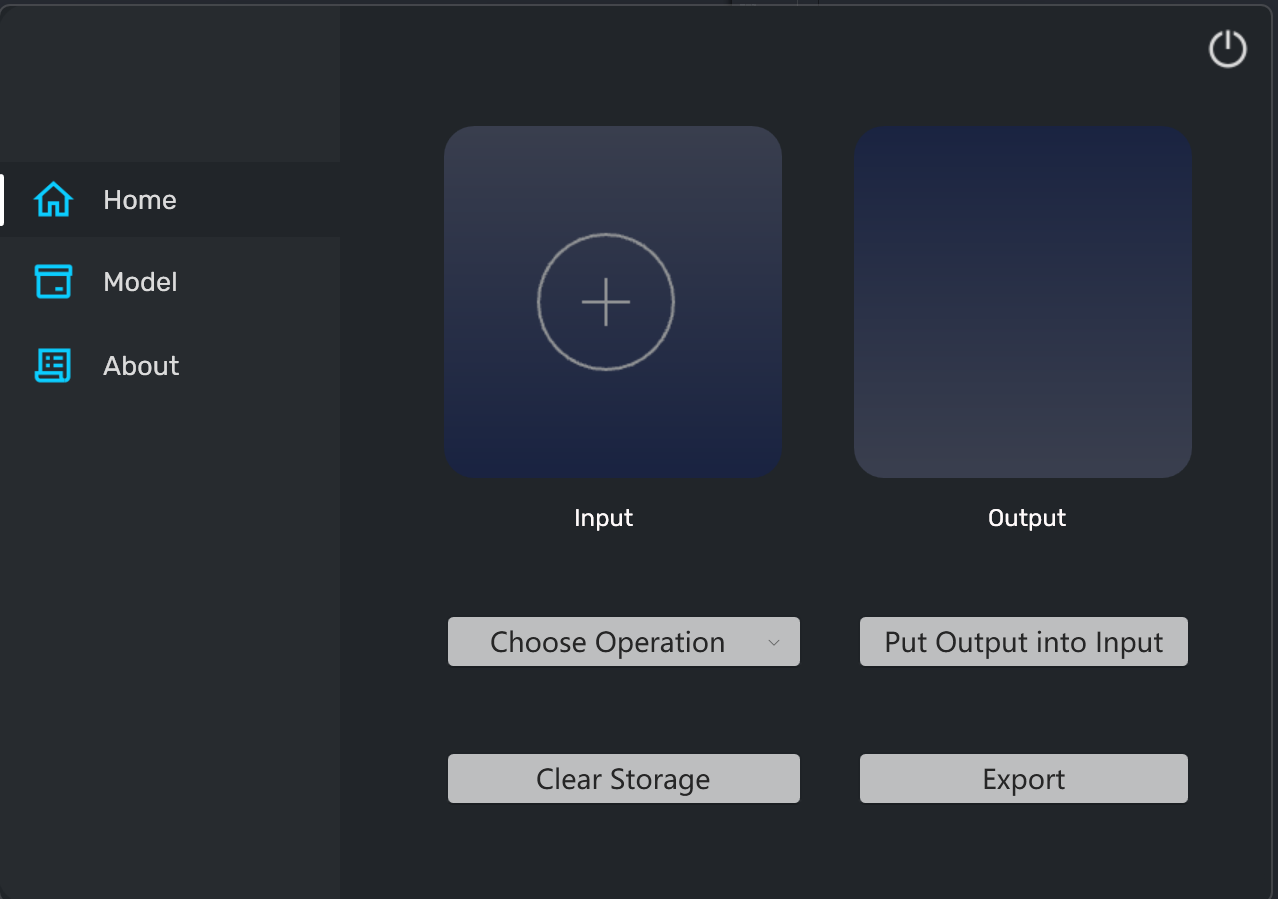
\includegraphics[width=0.8\textwidth]{img/image.png}
    \caption{连接到MySQL数据库}
\end{figure}

在终端1中,运行以下命令:

\begin{lstlisting}[language=sql]
show global variables like 'autocommit'; 
show session variables like 'autocommit'; 
show global variables like '%transaction%'; 
show session variables like '%transaction%'; 
set global autocommit = OFF; 
set session autocommit = OFF; 
select @@global.autocommit, @@session.autocommit; 
\end{lstlisting}

可以得到以下结果:

\begin{lstlisting}[language=sql]
mysql> show session variables like 'autocommit';
+---------------+-------+
| Variable_name | Value |
+---------------+-------+
| autocommit    | ON    |
+---------------+-------+
1 row in set (0.07 sec)

mysql> show global variables like '%transaction%';
+----------------------------------------------------------+-----------------+
| Variable_name                                            | Value           |
+----------------------------------------------------------+-----------------+
| binlog_direct_non_transactional_updates                  | OFF             |
| binlog_transaction_compression                           | OFF             |
| binlog_transaction_compression_level_zstd                | 3               |
| binlog_transaction_dependency_history_size               | 25000           |
| binlog_transaction_dependency_tracking                   | COMMIT_ORDER    |
| performance_schema_events_transactions_history_long_size | 10000           |
| performance_schema_events_transactions_history_size      | 10              |
| replica_transaction_retries                              | 10              |
| session_track_transaction_info                           | OFF             |
| slave_transaction_retries                                | 10              |
| transaction_alloc_block_size                             | 8192            |
| transaction_isolation                                    | REPEATABLE-READ |
| transaction_prealloc_size                                | 4096            |
| transaction_read_only                                    | OFF             |
| transaction_write_set_extraction                         | XXHASH64        |
+----------------------------------------------------------+-----------------+
15 rows in set (0.00 sec)

mysql> show session variables like '%transaction%';
+----------------------------------------------------------+-----------------+
| Variable_name                                            | Value           |
+----------------------------------------------------------+-----------------+
| binlog_direct_non_transactional_updates                  | OFF             |
| binlog_transaction_compression                           | OFF             |
| binlog_transaction_compression_level_zstd                | 3               |
| binlog_transaction_dependency_history_size               | 25000           |
| binlog_transaction_dependency_tracking                   | COMMIT_ORDER    |
| performance_schema_events_transactions_history_long_size | 10000           |
| performance_schema_events_transactions_history_size      | 10              |
| replica_transaction_retries                              | 10              |
| session_track_transaction_info                           | OFF             |
| slave_transaction_retries                                | 10              |
| transaction_alloc_block_size                             | 8192            |
| transaction_allow_batching                               | OFF             |
| transaction_isolation                                    | REPEATABLE-READ |
| transaction_prealloc_size                                | 4096            |
| transaction_read_only                                    | OFF             |
| transaction_write_set_extraction                         | XXHASH64        |
+----------------------------------------------------------+-----------------+
16 rows in set (0.00 sec)

mysql> set global autocommit = OFF;
Query OK, 0 rows affected (0.00 sec)

mysql> set session autocommit = OFF;
Query OK, 0 rows affected (0.00 sec)

mysql> select @@global.autocommit, @@session.autocommit;
+---------------------+----------------------+
| @@global.autocommit | @@session.autocommit |
+---------------------+----------------------+
|                   0 |                    0 |
+---------------------+----------------------+
1 row in set (0.00 sec)
\end{lstlisting}

在终端2中,运行以下命令:

\begin{lstlisting}[language=sql]
select @@global.autocommit, @@session.autocommit;
\end{lstlisting}

可以得到以下结果:

\begin{lstlisting}[language=sql]
mysql> select @@global.autocommit, @@session.autocommit;
+---------------------+----------------------+
| @@global.autocommit | @@session.autocommit |
+---------------------+----------------------+
|                   0 |                    1 |
+---------------------+----------------------+
1 row in set (0.00 sec)
\end{lstlisting}

说明目前终端1的会话中的autocommit为OFF,而终端2的会话中的autocommit为ON。

在终端1、2、3中,分别按照顺序运行以下命令:

\begin{lstlisting}[language=sql]
insert into region values(5,'MOON','Inserted by a non-autocommit transaction.'); -- T1
insert into region values(6,'SUN','Inserted by an autocommit transaction.'); -- T2
start transaction; -- T3
insert into region values(7,'STAR','Inserted by a rollback transaction.'); -- T3
select * from region; -- T1
select * from region; -- T2
select * from region; -- T3
commit; -- T1
rollback; -- T3
select * from region; -- T1
select * from region; -- T2
select * from region; -- T3
\end{lstlisting}

得到结果:

T1:

\begin{lstlisting}[language=sql]
mysql> insert into region values(5,'MOON','Inserted by a non-autocommit transaction.');
Query OK, 1 row affected (0.04 sec)

mysql> select * from region;

| r_regionkey | r_name      | r_comment
                          |

|           0 | AFRICA      | lar deposits. blithely final packages cajole. regular waters are final requests. regular accounts are according to  |
|           1 | AMERICA     | hs use ironic, even requests. s
                          |
|           2 | ASIA        | ges. thinly even pinto beans ca
                          |
|           3 | EUROPE      | ly final courts cajole furiously final excuse
                          |
|           4 | MIDDLE EAST | uickly special accounts cajole carefully blithely close requests. carefully final asymptotes haggle furiousl        |
|           5 | MOON        | Inserted by a non-autocommit transaction.
                          |
|           6 | SUN         | Inserted by an autocommit transaction.
                          |

7 rows in set (0.00 sec)

mysql> commit;
Query OK, 0 rows affected (0.01 sec)

mysql> select * from region;

| r_regionkey | r_name      | r_comment
                          |

|           0 | AFRICA      | lar deposits. blithely final packages cajole. regular waters are final requests. regular accounts are according to  |
|           1 | AMERICA     | hs use ironic, even requests. s
                          |
|           2 | ASIA        | ges. thinly even pinto beans ca
                          |
|           3 | EUROPE      | ly final courts cajole furiously final excuse
                          |
|           4 | MIDDLE EAST | uickly special accounts cajole carefully blithely close requests. carefully final asymptotes haggle furiousl        |
|           5 | MOON        | Inserted by a non-autocommit transaction.
                          |
|           6 | SUN         | Inserted by an autocommit transaction.
                          |

7 rows in set (0.00 sec)
\end{lstlisting}

T2:

可以看出,T1需要手动提交,T2自动提交。

在终端1、2、3中,分别按照顺序运行以下命令:

\begin{lstlisting}[language=sql]
start transaction; -- T2
delete from region where r_regionkey = 6; -- T2
select * from region; -- T1
select * from region; -- T2
select * from region; -- T3
rollback; -- T2
select * from region; -- T1
select * from region; -- T2
select * from region; -- T3
start transaction; -- T2
delete from region where r_regionkey = 6; -- T2
select * from region; -- T1
select * from region; -- T2
select * from region; -- T3
analyze table orders; -- T2
rollback; -- T2
select * from region; -- T1
select * from region; -- T2
select * from region; -- T3
commit; --T1
\end{lstlisting}

其中,T1的终端输出为:

\begin{lstlisting}[language=sql]
mysql> select * from region;

| r_regionkey | r_name      | r_comment
                          |

|           0 | AFRICA      | lar deposits. blithely final packages cajole. regular waters are final requests. regular accounts are according to  |
|           1 | AMERICA     | hs use ironic, even requests. s
                          |
|           2 | ASIA        | ges. thinly even pinto beans ca
                          |
|           3 | EUROPE      | ly final courts cajole furiously final excuse
                          |
|           4 | MIDDLE EAST | uickly special accounts cajole carefully blithely close requests. carefully final asymptotes haggle furiousl        |
|           5 | MOON        | Inserted by a non-autocommit transaction.
                          |
|           6 | SUN         | Inserted by an autocommit transaction.
                          |

7 rows in set (0.00 sec)

mysql> select * from region;

| r_regionkey | r_name      | r_comment
                          |

|           0 | AFRICA      | lar deposits. blithely final packages cajole. regular waters are final requests. regular accounts are according to  |
|           1 | AMERICA     | hs use ironic, even requests. s
                          |
|           2 | ASIA        | ges. thinly even pinto beans ca
                          |
|           3 | EUROPE      | ly final courts cajole furiously final excuse
                          |
|           4 | MIDDLE EAST | uickly special accounts cajole carefully blithely close requests. carefully final asymptotes haggle furiousl        |
|           5 | MOON        | Inserted by a non-autocommit transaction.
                          |
|           6 | SUN         | Inserted by an autocommit transaction.
                          |

7 rows in set (0.00 sec)

mysql> select * from region;

| r_regionkey | r_name      | r_comment
                          |

|           0 | AFRICA      | lar deposits. blithely final packages cajole. regular waters are final requests. regular accounts are according to  |
|           1 | AMERICA     | hs use ironic, even requests. s
                          |
|           2 | ASIA        | ges. thinly even pinto beans ca
                          |
|           3 | EUROPE      | ly final courts cajole furiously final excuse
                          |
|           4 | MIDDLE EAST | uickly special accounts cajole carefully blithely close requests. carefully final asymptotes haggle furiousl        |
|           5 | MOON        | Inserted by a non-autocommit transaction.
                          |
|           6 | SUN         | Inserted by an autocommit transaction.
                          |

7 rows in set (0.00 sec)

mysql> select * from region;

| r_regionkey | r_name      | r_comment
                          |

|           0 | AFRICA      | lar deposits. blithely final packages cajole. regular waters are final requests. regular accounts are according to  |
|           1 | AMERICA     | hs use ironic, even requests. s
                          |
|           2 | ASIA        | ges. thinly even pinto beans ca
                          |
|           3 | EUROPE      | ly final courts cajole furiously final excuse
                          |
|           4 | MIDDLE EAST | uickly special accounts cajole carefully blithely close requests. carefully final asymptotes haggle furiousl        |
|           5 | MOON        | Inserted by a non-autocommit transaction.
                          |
|           6 | SUN         | Inserted by an autocommit transaction.
                          |

7 rows in set (0.00 sec)

mysql> commit;
Query OK, 0 rows affected (0.00 sec)

\end{lstlisting}

T2的终端输出为:

\begin{lstlisting}[language=sql]
mysql> select * from region;
 
| r_regionkey | r_name      | r_comment
                          |
 
|           0 | AFRICA      | lar deposits. blithely final packages cajole. regular waters are final requests. regular accounts are according to  |
|           1 | AMERICA     | hs use ironic, even requests. s
                          |
|           2 | ASIA        | ges. thinly even pinto beans ca
                          |
|           3 | EUROPE      | ly final courts cajole furiously final excuse
                          |
|           4 | MIDDLE EAST | uickly special accounts cajole carefully blithely close requests. carefully final asymptotes haggle furiousl        |
|           5 | MOON        | Inserted by a non-autocommit transaction.
                          |
 
6 rows in set (0.00 sec)

mysql> rollback;
Query OK, 0 rows affected (0.01 sec)

mysql> select * from region;
 
| r_regionkey | r_name      | r_comment
                          |
 
|           0 | AFRICA      | lar deposits. blithely final packages cajole. regular waters are final requests. regular accounts are according to  |
|           1 | AMERICA     | hs use ironic, even requests. s
                          |
|           2 | ASIA        | ges. thinly even pinto beans ca
                          |
|           3 | EUROPE      | ly final courts cajole furiously final excuse
                          |
|           4 | MIDDLE EAST | uickly special accounts cajole carefully blithely close requests. carefully final asymptotes haggle furiousl        |
|           5 | MOON        | Inserted by a non-autocommit transaction.
                          |
|           6 | SUN         | Inserted by an autocommit transaction.
                          |

7 rows in set (0.00 sec)

mysql> start transaction;
Query OK, 0 rows affected (0.00 sec)

mysql> delete from region where r_regionkey = 6;
Query OK, 1 row affected (0.01 sec)

mysql> select * from region;

| r_regionkey | r_name      | r_comment
                          |

|           0 | AFRICA      | lar deposits. blithely final packages cajole. regular waters are final requests. regular accounts are according to  |
|           1 | AMERICA     | hs use ironic, even requests. s
                          |
|           2 | ASIA        | ges. thinly even pinto beans ca
                          |
|           3 | EUROPE      | ly final courts cajole furiously final excuse
                          |
|           4 | MIDDLE EAST | uickly special accounts cajole carefully blithely close requests. carefully final asymptotes haggle furiousl        |
|           5 | MOON        | Inserted by a non-autocommit transaction.
                          |

6 rows in set (0.00 sec)

mysql> analyze table orders;
+-------------+---------+----------+----------+
| Table       | Op      | Msg_type | Msg_text |
+-------------+---------+----------+----------+
| tpch.orders | analyze | status   | OK       |
+-------------+---------+----------+----------+
1 row in set (0.08 sec)

mysql> rollback;
Query OK, 0 rows affected (0.00 sec)

mysql> select * from region;

| r_regionkey | r_name      | r_comment
                          |

|           0 | AFRICA      | lar deposits. blithely final packages cajole. regular waters are final requests. regular accounts are according to  |
|           1 | AMERICA     | hs use ironic, even requests. s
                          |
|           2 | ASIA        | ges. thinly even pinto beans ca
                          |
|           3 | EUROPE      | ly final courts cajole furiously final excuse
                          |
|           4 | MIDDLE EAST | uickly special accounts cajole carefully blithely close requests. carefully final asymptotes haggle furiousl        |
|           5 | MOON        | Inserted by a non-autocommit transaction.

6 rows in set (0.00 sec)
\end{lstlisting}

T3的终端输出为:

\begin{lstlisting}[language=sql]
mysql> select * from region;
  
| r_regionkey | r_name      | r_comment 
  
|           0 | AFRICA      | lar deposits. blithely final packages cajole. regular waters are final requests. regular accounts are according to  |
|           1 | AMERICA     | hs use ironic, even requests. s
                          |
|           2 | ASIA        | ges. thinly even pinto beans ca
                          |
|           3 | EUROPE      | ly final courts cajole furiously final excuse
                          |
|           4 | MIDDLE EAST | uickly special accounts cajole carefully blithely close requests. carefully final asymptotes haggle furiousl        |
|           5 | MOON        | Inserted by a non-autocommit transaction.
                          |
|           6 | SUN         | Inserted by an autocommit transaction.
                          |
  
7 rows in set (0.00 sec)

mysql> select * from region;
  
| r_regionkey | r_name      | r_comment
                          |
  
|           0 | AFRICA      | lar deposits. blithely final packages cajole. regular waters are final requests. regular accounts are according to  |
|           1 | AMERICA     | hs use ironic, even requests. s
                          |
|           2 | ASIA        | ges. thinly even pinto beans ca
                          |
|           3 | EUROPE      | ly final courts cajole furiously final excuse
                          |
|           4 | MIDDLE EAST | uickly special accounts cajole carefully blithely close requests. carefully final asymptotes haggle furiousl        |
|           5 | MOON        | Inserted by a non-autocommit transaction.
                          |
|           6 | SUN         | Inserted by an autocommit transaction.
                          |
  
7 rows in set (0.00 sec)

mysql> select * from region;
  
| r_regionkey | r_name      | r_comment
                          |
  
|           0 | AFRICA      | lar deposits. blithely final packages cajole. regular waters are final requests. regular accounts are according to  |
|           1 | AMERICA     | hs use ironic, even requests. s
                          |
|           2 | ASIA        | ges. thinly even pinto beans ca
                          |
|           3 | EUROPE      | ly final courts cajole furiously final excuse
                          |
|           4 | MIDDLE EAST | uickly special accounts cajole carefully blithely close requests. carefully final asymptotes haggle furiousl        |
|           5 | MOON        | Inserted by a non-autocommit transaction.
                          |
|           6 | SUN         | Inserted by an autocommit transaction.
                          |
  
7 rows in set (0.00 sec)

mysql> select * from region;
  
| r_regionkey | r_name      | r_comment
                          |
  
|           0 | AFRICA      | lar deposits. blithely final packages cajole. regular waters are final requests. regular accounts are according to  |
|           1 | AMERICA     | hs use ironic, even requests. s
                          |
|           2 | ASIA        | ges. thinly even pinto beans ca
                          |
|           3 | EUROPE      | ly final courts cajole furiously final excuse
                          |
|           4 | MIDDLE EAST | uickly special accounts cajole carefully blithely close requests. carefully final asymptotes haggle furiousl        |
|           5 | MOON        | Inserted by a non-autocommit transaction.
                          |
  
6 rows in set (0.01 sec)
\end{lstlisting}

因此,调用analyze table orders语句后,T2将提交,因此不会回滚。

在客户端T2中执行下列语句,关注使用SAVEPOINT:

\begin{lstlisting}[language=sql]
start transaction;
insert into region values(5,'MOON','Savepoint moon');
savepoint moon;
insert into region values(6,'SUN','Savepoint sun');
savepoint sun;
insert into region values(7,'STAR','Savepoint star');
savepoint star;
select * from region;
rollback to sun;
select * from region;
rollback to star;
select * from region;
rollback to moon;
select * from region;
commit;
\end{lstlisting}

可以在T2中得到以下结果:

\begin{lstlisting}[language=sql]
mysql> start transaction;
Query OK, 0 rows affected (0.00 sec)

mysql> insert into region values(5,'MOON','Savepoint moon');
ERROR 1062 (23000): Duplicate entry '5' for key 'region.PRIMARY'
mysql> savepoint moon;
Query OK, 0 rows affected (0.00 sec)

mysql> insert into region values(6,'SUN','Savepoint sun');
Query OK, 1 row affected (0.00 sec)

mysql> savepoint sun;
Query OK, 0 rows affected (0.00 sec)

mysql> insert into region values(7,'STAR','Savepoint star');
Query OK, 1 row affected (0.00 sec)

mysql> savepoint star;
Query OK, 0 rows affected (0.00 sec)

mysql> select * from region;
   
| r_regionkey | r_name      | r_comment
                          |
   
|           0 | AFRICA      | lar deposits. blithely final packages cajole. regular waters are final requests. regular accounts are according to  |
|           1 | AMERICA     | hs use ironic, even requests. s
                          |
|           2 | ASIA        | ges. thinly even pinto beans ca
                          |
|           3 | EUROPE      | ly final courts cajole furiously final excuse
                          |
|           4 | MIDDLE EAST | uickly special accounts cajole carefully blithely close requests. carefully final asymptotes haggle furiousl        |
|           5 | MOON        | Inserted by a non-autocommit transaction.
                          |
|           6 | SUN         | Savepoint sun
                          |
|           7 | STAR        | Savepoint star
                          |
   
8 rows in set (0.01 sec)

mysql> rollback to sun;
Query OK, 0 rows affected (0.00 sec)

mysql> select * from region;
   
| r_regionkey | r_name      | r_comment
                          |
   
|           0 | AFRICA      | lar deposits. blithely final packages cajole. regular waters are final requests. regular accounts are according to  |
|           1 | AMERICA     | hs use ironic, even requests. s
                          |
|           2 | ASIA        | ges. thinly even pinto beans ca
                          |
|           3 | EUROPE      | ly final courts cajole furiously final excuse
                          |
|           4 | MIDDLE EAST | uickly special accounts cajole carefully blithely close requests. carefully final asymptotes haggle furiousl        |
|           5 | MOON        | Inserted by a non-autocommit transaction.
                          |
|           6 | SUN         | Savepoint sun
                          |
   
7 rows in set (0.00 sec)

mysql> rollback to star;
ERROR 1305 (42000): SAVEPOINT star does not exist
mysql> select * from region;
   
| r_regionkey | r_name      | r_comment
                          |
   
|           0 | AFRICA      | lar deposits. blithely final packages cajole. regular waters are final requests. regular accounts are according to  |
|           1 | AMERICA     | hs use ironic, even requests. s
                          |
|           2 | ASIA        | ges. thinly even pinto beans ca
                          |
|           3 | EUROPE      | ly final courts cajole furiously final excuse
                          |
|           4 | MIDDLE EAST | uickly special accounts cajole carefully blithely close requests. carefully final asymptotes haggle furiousl        |
|           5 | MOON        | Inserted by a non-autocommit transaction.
                          |
|           6 | SUN         | Savepoint sun
                          |
   
7 rows in set (0.00 sec)

mysql> rollback to moon;
Query OK, 0 rows affected (0.00 sec)

mysql> select * from region;
   
| r_regionkey | r_name      | r_comment
                          |
   
|           0 | AFRICA      | lar deposits. blithely final packages cajole. regular waters are final requests. regular accounts are according to  |
|           1 | AMERICA     | hs use ironic, even requests. s
                          |
|           2 | ASIA        | ges. thinly even pinto beans ca
                          |
|           3 | EUROPE      | ly final courts cajole furiously final excuse
                          |
|           4 | MIDDLE EAST | uickly special accounts cajole carefully blithely close requests. carefully final asymptotes haggle furiousl        |
|           5 | MOON        | Inserted by a non-autocommit transaction.
                          |
   
6 rows in set (0.00 sec)

mysql> commit;
Query OK, 0 rows affected (0.02 sec)
\end{lstlisting}

因此,可以看出,SAVEPOINT的作用是在事务中设置一个回滚点,可以在回滚时回滚到这个点。

分别在不同客户端中执行下列语句,关注使用LOCK TABLES语句:

\begin{lstlisting}[language=sql]
lock tables region read; -- T2
select count(*) from region; -- T2
select count(*) from nation; -- T2
select * from region; -- T3
delete from region where r_regionkey = 5; -- T3
lock tables nation write, nation as n1 read; -- T2
insert into nation select n_nationkey+100, n_name, n_regionkey,n_comment from nation; -- T2;
insert into nation select n_nationkey+100, n_name, n_regionkey,n_comment from nation as n1; -- T2;
lock tables region read; -- T2
select * from region; -- T2
select * from region as r; -- T2
lock tables region as r read; -- T2
select * from region; -- T2
select * from region as r; -- T2
delete from nation where n_nationkey >= 100; -- T3
\end{lstlisting}

可以在T2中得到以下结果:

\begin{lstlisting}[language=sql]
mysql> lock tables region read; -- T2
Query OK, 0 rows affected (0.00 sec)

mysql> select count(*) from region; -- T2
+----------+
| count(*) |
+----------+
|        6 |
+----------+
1 row in set (0.00 sec)

mysql> select count(*) from nation; -- T2
ERROR 1100 (HY000): Table 'nation' was not locked with LOCK TABLES
mysql> lock tables nation write, nation as n1 read; -- T2
Query OK, 0 rows affected (0.00 sec)

mysql> insert into nation select n_nationkey+100, n_name, n_regionkey,n_comment from nation; -- T2;
ERROR 1100 (HY000): Table 'nation' was not locked with LOCK TABLES
mysql> insert into nation select n_nationkey+100, n_name, n_regionkey,n_comment from nation as n1; -- T2;
Query OK, 25 rows affected (0.09 sec)
Records: 25  Duplicates: 0  Warnings: 0

mysql> lock tables region read; -- T2
Query OK, 0 rows affected (0.00 sec)

mysql> select * from region; -- T2
    
| r_regionkey | r_name      | r_comment
                          |
    
|           0 | AFRICA      | lar deposits. blithely final packages cajole. regular waters are final requests. regular accounts are according to  |
|           1 | AMERICA     | hs use ironic, even requests. s
                          |
|           2 | ASIA        | ges. thinly even pinto beans ca
                          |
|           3 | EUROPE      | ly final courts cajole furiously final excuse
                          |
|           4 | MIDDLE EAST | uickly special accounts cajole carefully blithely close requests. carefully final asymptotes haggle furiousl        |
    
5 rows in set (0.00 sec)

mysql> select * from region as r; -- T2
ERROR 1100 (HY000): Table 'r' was not locked with LOCK TABLES
mysql> lock tables region as r read; -- T2
Query OK, 0 rows affected (0.00 sec)

mysql> select * from region; -- T2
ERROR 1100 (HY000): Table 'region' was not locked with LOCK TABLES
mysql> select * from region as r; -- T2
    
| r_regionkey | r_name      | r_comment
                          |
    
|           0 | AFRICA      | lar deposits. blithely final packages cajole. regular waters are final requests. regular accounts are according to  |
|           1 | AMERICA     | hs use ironic, even requests. s
                          |
|           2 | ASIA        | ges. thinly even pinto beans ca
                          |
|           3 | EUROPE      | ly final courts cajole furiously final excuse
                          |
|           4 | MIDDLE EAST | uickly special accounts cajole carefully blithely close requests. carefully final asymptotes haggle furiousl        |
    
5 rows in set (0.00 sec)
\end{lstlisting}

可以在T3中得到以下结果:

\begin{lstlisting}[language=sql]
mysql> select * from region; -- T3

| r_regionkey | r_name      | r_comment
                          |

|           0 | AFRICA      | lar deposits. blithely final packages cajole. regular waters are final requests. regular accounts are according to  |
|           1 | AMERICA     | hs use ironic, even requests. s
                          |
|           2 | ASIA        | ges. thinly even pinto beans ca
                          |
|           3 | EUROPE      | ly final courts cajole furiously final excuse
                          |
|           4 | MIDDLE EAST | uickly special accounts cajole carefully blithely close requests. carefully final asymptotes haggle furiousl        |
|           5 | MOON        | Inserted by a non-autocommit transaction.
                          |

6 rows in set (0.00 sec)

mysql> delete from region where r_regionkey = 5; -- T3
Query OK, 1 row affected (45.59 sec)

mysql> delete from nation where n_nationkey >= 100;
Query OK, 25 rows affected (0.01 sec)
\end{lstlisting}

因此,可以得知,LOCK TABLES语句可以锁定表,使得其他事务无法对其进行操作。

在客户端T2中执行下列语句:

\begin{lstlisting}[language=sql]
mysql> select @@global.transaction_isolation, @@global.transaction_read_only;
+--------------------------------+--------------------------------+
| @@global.transaction_isolation | @@global.transaction_read_only |
+--------------------------------+--------------------------------+
| REPEATABLE-READ                |                              0 |
+--------------------------------+--------------------------------+
1 row in set (0.00 sec)

mysql> set global transaction isolation level serializable;
Query OK, 0 rows affected (0.02 sec)

mysql> set global transaction read only;
Query OK, 0 rows affected (0.00 sec)

mysql> select @@global.transaction_isolation, @@global.transaction_read_only;
+--------------------------------+--------------------------------+
| @@global.transaction_isolation | @@global.transaction_read_only |
+--------------------------------+--------------------------------+
| SERIALIZABLE                   |                              1 |
+--------------------------------+--------------------------------+
1 row in set (0.00 sec)

mysql> select @@session.transaction_isolation, @@session.transaction_read_only;
+---------------------------------+---------------------------------+
| @@session.transaction_isolation | @@session.transaction_read_only |
+---------------------------------+---------------------------------+
| REPEATABLE-READ                 |                               0 |
+---------------------------------+---------------------------------+
1 row in set (0.00 sec)

mysql> set @@session.transaction_isolation = 'read-committed';
Query OK, 0 rows affected (0.00 sec)

mysql> set @@session.transaction_read_only = on;
Query OK, 0 rows affected (0.00 sec)

mysql> select @@session.transaction_isolation, @@session.transaction_read_only;
+---------------------------------+---------------------------------+
| @@session.transaction_isolation | @@session.transaction_read_only |
+---------------------------------+---------------------------------+
| READ-COMMITTED                  |                               1 |
+---------------------------------+---------------------------------+
1 row in set (0.00 sec)

mysql> start transaction;
Query OK, 0 rows affected (0.00 sec)

mysql> select * from region;
    
| r_regionkey | r_name      | r_comment
                          |
    
|           0 | AFRICA      | lar deposits. blithely final packages cajole. regular waters are final requests. regular accounts are according to  |
|           1 | AMERICA     | hs use ironic, even requests. s
                          |
|           2 | ASIA        | ges. thinly even pinto beans ca
                          |
|           3 | EUROPE      | ly final courts cajole furiously final excuse
                          |
|           4 | MIDDLE EAST | uickly special accounts cajole carefully blithely close requests. carefully final asymptotes haggle furiousl        |
    
5 rows in set (0.00 sec)

mysql> insert into region values(5,'MOON','Read only?');
ERROR 1792 (25006): Cannot execute statement in a READ ONLY transaction.
mysql> set transaction_read_only = off;
Query OK, 0 rows affected (0.00 sec)

mysql>
mysql> insert into region values(5,'MOON','Read only?');
ERROR 1792 (25006): Cannot execute statement in a READ ONLY transaction.
mysql> commit;
Query OK, 0 rows affected (0.00 sec)

mysql> start transaction;
Query OK, 0 rows affected (0.00 sec)

mysql> select * from region;
    
| r_regionkey | r_name      | r_comment
                          |
    
|           0 | AFRICA      | lar deposits. blithely final packages cajole. regular waters are final requests. regular accounts are according to  |
|           1 | AMERICA     | hs use ironic, even requests. s
                          |
|           2 | ASIA        | ges. thinly even pinto beans ca
                          |
|           3 | EUROPE      | ly final courts cajole furiously final excuse
                          |
|           4 | MIDDLE EAST | uickly special accounts cajole carefully blithely close requests. carefully final asymptotes haggle furiousl        |
    
5 rows in set (0.00 sec)

mysql> insert into region values(5,'MOON','Read only?');
Query OK, 1 row affected (0.00 sec)

mysql> rollback;
Query OK, 0 rows affected (0.01 sec)

mysql> start transaction;
Query OK, 0 rows affected (0.00 sec)

mysql> select @@global.transaction_isolation, @@session.transaction_isolation;
+--------------------------------+---------------------------------+
| @@global.transaction_isolation | @@session.transaction_isolation |
+--------------------------------+---------------------------------+
| SERIALIZABLE                   | READ-COMMITTED                  |
+--------------------------------+---------------------------------+
1 row in set (0.00 sec)

mysql> set transaction isolation level serializable;
ERROR 1568 (25001): Transaction characteristics can't be changed while a transaction is in progress
mysql> select @@global.transaction_isolation, @@session.transaction_isolation;
+--------------------------------+---------------------------------+
| @@global.transaction_isolation | @@session.transaction_isolation |
+--------------------------------+---------------------------------+
| SERIALIZABLE                   | READ-COMMITTED                  |
+--------------------------------+---------------------------------+
1 row in set (0.00 sec)

mysql> set session transaction isolation level serializable;
Query OK, 0 rows affected (0.00 sec)

mysql> select @@global.transaction_isolation, @@session.transaction_isolation;
+--------------------------------+---------------------------------+
| @@global.transaction_isolation | @@session.transaction_isolation |
+--------------------------------+---------------------------------+
| SERIALIZABLE                   | SERIALIZABLE                    |
+--------------------------------+---------------------------------+
1 row in set (0.00 sec)

mysql> commit;
Query OK, 0 rows affected (0.00 sec)
\end{lstlisting}

因此,通过设置transaction isolation level和transaction read only,可以设置事务的隔离级别和只读属性。

分别在不同客户端中执行下列语句,关注查询事务的状态:

\begin{lstlisting}[language=sql]
set innodb_lock_wait_timeout = 600; -- T1
set innodb_lock_wait_timeout = 600; -- T2
set innodb_lock_wait_timeout = 600; -- T3
set session transaction isolation level read committed; -- T1
start transaction; -- T1
set session transaction isolation level repeatable read; -- T2
start transaction; -- T2
set session transaction isolation level serializable;
start transaction; -- T3
select trx_id, trx_state, trx_isolation_level, trx_is_read_only from information_schema.innodb_trx; -- T1
select * from performance_schema.processlist; -- T1
select * from performance_schema.data_locks; -- T1
select * from region; -- T1
select * from nation limit 5; -- T2
select * from customer limit 5; -- T3
select trx_id, trx_state, trx_isolation_level, trx_is_read_only from
information_schema.innodb_trx; -- T1
select * from performance_schema.processlist; -- T1
select engine_transaction_id, thread_id, object_schema, object_name,
lock_type, lock_mode, lock_data from performance_schema.data_locks; -- T1
insert into nation values(8888,'TEST',1,'It is a test.'); -- T1
update nation set n_comment = 'It is a test.' where n_nationkey = 0; -- T1
insert into customer values(99999,'Nobody','Nowhere',10,'12345678',3.14,'BUILDING','It is a test.'); -- T2
update customer set c_comment = 'It is a test.' where c_custkey = 1; -- T2
insert into region values(5,'MOON','It is a test'); -- T3
update region set r_comment = 'It is a test.' where r_regionkey = 0; -- T3
select trx_id, trx_state, trx_isolation_level, trx_is_read_only from information_schema.innodb_trx; -- T1
select * from performance_schema.processlist; -- T1
select engine_transaction_id, thread_id, object_schema, object_name, lock_type, lock_mode, lock_data from performance_schema.data_locks; -- T1
SELECT r.trx_id waiting_trx_id, r.trx_mysql_thread_id waiting_thread, r.trx_query waiting_query, b.trx_id blocking_trx_id, b.trx_mysql_thread_id blocking_thread, b.trx_query blocking_query FROM performance_schema.data_lock_waits w INNER JOIN information_schema.innodb_trx b ON b.trx_id = w.blocking_engine_transaction_id INNER JOIN information_schema.innodb_trx r ON r.trx_id = w.requesting_engine_transaction_id; -- T1
SELECT waiting_trx_id, waiting_pid, waiting_query, blocking_trx_id, blocking_pid, blocking_query FROM sys.innodb_lock_waits; -- T1
rollback; -- T3
rollback; -- T2
rollback; -- T1
\end{lstlisting}

可以在T1中得到以下结果:

\begin{lstlisting}[language=sql]
mysql> set innodb_lock_wait_timeout = 600;
Query OK, 0 rows affected (0.01 sec)

mysql> set session transaction isolation level read committed; -- T1
Query OK, 0 rows affected (0.00 sec)

mysql> start transaction; -- T1
Query OK, 0 rows affected (0.01 sec)

mysql> select trx_id, trx_state, trx_isolation_level, trx_is_read_only from information_schema.innodb_trx; -- T1
+-----------------+-----------+---------------------+------------------+
| trx_id          | trx_state | trx_isolation_level | trx_is_read_only |
+-----------------+-----------+---------------------+------------------+
| 421426146312192 | RUNNING   | REPEATABLE READ     |                0 |
| 421426146311384 | RUNNING   | REPEATABLE READ     |                0 |
+-----------------+-----------+---------------------+------------------+
2 rows in set (0.01 sec)

mysql> select * from performance_schema.processlist; -- T1
    
| ID | USER            | HOST             | DB       | COMMAND | TIME  | STATE                  | INFO
                             | EXECUTION_ENGINE |
    
|  5 | event_scheduler | localhost        | NULL     | Daemon  | 10720 | Waiting on empty queue | NULL
                             | PRIMARY          |
| 10 | root            | localhost        | tpch     | Query   |     0 | executing              | select * from performance_schema.processlist -- T1 | PRIMARY          |
| 11 | root            | localhost        | tpch     | Sleep   |    14 |                        | NULL
                             | PRIMARY          |
| 12 | root            | localhost        | tpch     | Sleep   |     7 |                        | NULL
                             | PRIMARY          |
| 13 | root            | 172.17.0.1:42606 | dbcourse | Sleep   |  7783 |                        | NULL
                             | PRIMARY          |
| 14 | root            | 172.17.0.1:42612 | dbcourse | Sleep   |  7783 |                        | NULL
                             | PRIMARY          |
    
6 rows in set (0.03 sec)

mysql> select * from performance_schema.data_locks; -- T1
Empty set (0.01 sec)

mysql> select * from region; -- T1
    
| r_regionkey | r_name      | r_comment
                          |
    
|           0 | AFRICA      | lar deposits. blithely final packages cajole. regular waters are final requests. regular accounts are according to  |
|           1 | AMERICA     | hs use ironic, even requests. s
                          |
|           2 | ASIA        | ges. thinly even pinto beans ca
                          |
|           3 | EUROPE      | ly final courts cajole furiously final excuse
                          |
|           4 | MIDDLE EAST | uickly special accounts cajole carefully blithely close requests. carefully final asymptotes haggle furiousl        |
    
5 rows in set (0.01 sec)

mysql> select trx_id, trx_state, trx_isolation_level, trx_is_read_only from
    -> information_schema.innodb_trx; -- T1
+-----------------+-----------+---------------------+------------------+
| trx_id          | trx_state | trx_isolation_level | trx_is_read_only |
+-----------------+-----------+---------------------+------------------+
| 421426146314616 | RUNNING   | SERIALIZABLE        |                0 |
| 421426146313808 | RUNNING   | READ COMMITTED      |                0 |
| 421426146313000 | RUNNING   | REPEATABLE READ     |                0 |
| 421426146312192 | RUNNING   | REPEATABLE READ     |                0 |
| 421426146311384 | RUNNING   | REPEATABLE READ     |                0 |
+-----------------+-----------+---------------------+------------------+
5 rows in set (0.00 sec)

mysql> select * from performance_schema.processlist; -- T1
    
| ID | USER            | HOST             | DB       | COMMAND | TIME  | STATE                  | INFO
                             | EXECUTION_ENGINE |
    
|  5 | event_scheduler | localhost        | NULL     | Daemon  | 10743 | Waiting on empty queue | NULL
                             | PRIMARY          |
| 10 | root            | localhost        | tpch     | Query   |     0 | executing              | select * from performance_schema.processlist -- T1 | PRIMARY          |
| 11 | root            | localhost        | tpch     | Sleep   |    16 |                        | NULL
                             | PRIMARY          |
| 12 | root            | localhost        | tpch     | Sleep   |    12 |                        | NULL
                             | PRIMARY          |
| 13 | root            | 172.17.0.1:42606 | dbcourse | Sleep   |  7806 |                        | NULL
                             | PRIMARY          |
| 14 | root            | 172.17.0.1:42612 | dbcourse | Sleep   |  7806 |                        | NULL
                             | PRIMARY          |
    
6 rows in set (0.00 sec)

mysql> select engine_transaction_id, thread_id, object_schema, object_name,
    -> lock_type, lock_mode, lock_data from performance_schema.data_locks; -- T1
    
| engine_transaction_id | thread_id | object_schema | object_name | lock_type | lock_mode | lock_data |
    
|       421426146314616 |        53 | tpch          | customer    | TABLE     | IS        | NULL      |
|       421426146314616 |        53 | tpch          | customer    | RECORD    | S         | 1         |
|       421426146314616 |        53 | tpch          | customer    | RECORD    | S         | 2         |
|       421426146314616 |        53 | tpch          | customer    | RECORD    | S         | 3         |
|       421426146314616 |        53 | tpch          | customer    | RECORD    | S         | 4         |
|       421426146314616 |        53 | tpch          | customer    | RECORD    | S         | 5         |
    
6 rows in set (0.00 sec)

mysql> insert into nation values(8888,'TEST',1,'It is a test.'); -- T1
Query OK, 1 row affected (0.00 sec)

mysql> update nation set n_comment = 'It is a test.' where n_nationkey = 0; -- T1
Query OK, 1 row affected (0.01 sec)
Rows matched: 1  Changed: 1  Warnings: 0

mysql> select trx_id, trx_state, trx_isolation_level, trx_is_read_only from information_schema.innodb_trx; -- T1
+-----------------+-----------+---------------------+------------------+
| trx_id          | trx_state | trx_isolation_level | trx_is_read_only |
+-----------------+-----------+---------------------+------------------+
|           57183 | RUNNING   | SERIALIZABLE        |                0 |
|           57182 | LOCK WAIT | REPEATABLE READ     |                0 |
|           57181 | RUNNING   | READ COMMITTED      |                0 |
| 421426146312192 | RUNNING   | REPEATABLE READ     |                0 |
| 421426146311384 | RUNNING   | REPEATABLE READ     |                0 |
+-----------------+-----------+---------------------+------------------+
5 rows in set (0.00 sec)

mysql> select * from performance_schema.processlist; -- T1
    
| ID | USER            | HOST             | DB       | COMMAND | TIME  | STATE                  | INFO
                                                    | EXECUTION_ENGINE |
    
|  5 | event_scheduler | localhost        | NULL     | Daemon  | 10770 | Waiting on empty queue | NULL
                                                    | PRIMARY          |
| 10 | root            | localhost        | tpch     | Query   |     0 | executing              | select * from performance_schema.processlist -- T1                        | PRIMARY          |
| 11 | root            | localhost        | tpch     | Query   |    16 | updating               | update customer set c_comment = 'It is a test.' where c_custkey = 1 -- T2 | PRIMARY          |
| 12 | root            | localhost        | tpch     | Sleep   |     8 |                        | NULL
                                                    | PRIMARY          |
| 13 | root            | 172.17.0.1:42606 | dbcourse | Sleep   |  7833 |                        | NULL
                                                    | PRIMARY          |
| 14 | root            | 172.17.0.1:42612 | dbcourse | Sleep   |  7833 |                        | NULL
                                                    | PRIMARY          |
    
6 rows in set (0.00 sec)

mysql> select engine_transaction_id, thread_id, object_schema, object_name, lock_type, lock_mode, lock_data from performance_schema.data_locks; -- T1
    
| engine_transaction_id | thread_id | object_schema | object_name | lock_type | lock_mode     | lock_data |
    
|                 57183 |        53 | tpch          | region      | TABLE     | IX            | NULL      |
|                 57183 |        53 | tpch          | customer    | TABLE     | IS            | NULL      |
|                 57183 |        53 | tpch          | customer    | RECORD    | S             | 1         |
|                 57183 |        53 | tpch          | customer    | RECORD    | S             | 2         |
|                 57183 |        53 | tpch          | customer    | RECORD    | S             | 3         |
|                 57183 |        53 | tpch          | customer    | RECORD    | S             | 4         |
|                 57183 |        53 | tpch          | customer    | RECORD    | S             | 5         |
|                 57183 |        53 | tpch          | region      | RECORD    | S,REC_NOT_GAP | 5         |
|                 57183 |        53 | tpch          | region      | RECORD    | X,REC_NOT_GAP | 0         |
|                 57182 |        52 | tpch          | customer    | TABLE     | IX            | NULL      |
|                 57182 |        52 | tpch          | customer    | RECORD    | X,REC_NOT_GAP | 1         |
|                 57181 |        51 | tpch          | nation      | TABLE     | IX            | NULL      |
|                 57181 |        51 | tpch          | nation      | RECORD    | X,REC_NOT_GAP | 0         |
    
13 rows in set (0.00 sec)

mysql> SELECT r.trx_id waiting_trx_id, r.trx_mysql_thread_id waiting_thread, r.trx_query waiting_query, b.trx_id blocking_trx_id, b.trx_mysql_thread_id blocking_thread, b.trx_query blocking_query FROM performance_schema.data_lock_waits w INNER JOIN information_schema.innodb_trx b ON b.trx_id = w.blocking_engine_transaction_id INNER JOIN information_schema.innodb_trx r ON r.trx_id = w.requesting_engine_transaction_id; -- T1
    
| waiting_trx_id | waiting_thread | waiting_query                                                             | blocking_trx_id | blocking_thread | blocking_query |
    
|          57182 |             11 | update customer set c_comment = 'It is a test.' where c_custkey = 1 -- T2 |
  57183 |              12 | NULL           |
    
1 row in set (0.01 sec)

mysql> SELECT waiting_trx_id, waiting_pid, waiting_query, blocking_trx_id, blocking_pid, blocking_query FROM sys.innodb_lock_waits; -- T1
    
| waiting_trx_id | waiting_pid | waiting_query                                                     | blocking_trx_id | blocking_pid | blocking_query |
    
|          57182 |          11 | update customer set c_comment  ... st.' where c_custkey = 1 -- T2 |           57183 |           12 | NULL           |
    
1 row in set (0.04 sec)

mysql> rollback;
Query OK, 0 rows affected (0.01 sec)
\end{lstlisting}

可以在T2中得到以下结果:

\begin{lstlisting}[language=sql]
mysql> set innodb_lock_wait_timeout = 600;
Query OK, 0 rows affected (0.00 sec)

mysql> set session transaction isolation level repeatable read; -- T2
Query OK, 0 rows affected (0.00 sec)

mysql> start transaction; -- T2
Query OK, 0 rows affected (0.00 sec)

mysql> select * from nation limit 5; -- T2
    
| n_nationKEY | n_name    | n_regionkey | n_comment
                              |
    
|           0 | ALGERIA   |           0 |  haggle. carefully final deposits detect slyly agai
                              |
|           1 | ARGENTINA |           1 | al foxes promise slyly according to the regular accounts. bold requests alon                                |
|           2 | BRAZIL    |           1 | y alongside of the pending deposits. carefully special packages are about the ironic forges. slyly special  |
|           3 | CANADA    |           1 | eas hang ironic, silent packages. slyly regular packages are furiously over the tithes. fluffily bold       |
|           4 | EGYPT     |           4 | y above the carefully unusual theodolites. final dugouts are quickly across the furiously regular d         |
    
5 rows in set (0.00 sec)

mysql> insert into customer values(99999,'Nobody','Nowhere',10,'12345678',3.14,'BUILDING','It is a test.'); -- T2
Query OK, 1 row affected (0.02 sec)

mysql> update customer set c_comment = 'It is a test.' where c_custkey = 1; -- T2
Query OK, 1 row affected (25.16 sec)
Rows matched: 1  Changed: 1  Warnings: 0

mysql> rollback;
Query OK, 0 rows affected (0.02 sec)
\end{lstlisting}

可以在T3中得到以下结果:

\begin{lstlisting}[language=sql]
mysql> set innodb_lock_wait_timeout = 600;
Query OK, 0 rows affected (0.00 sec)

mysql> set session transaction isolation level serializable;
Query OK, 0 rows affected (0.00 sec)

mysql> start transaction; -- T3
Query OK, 0 rows affected (0.00 sec)

mysql> select * from customer limit 5; -- T3
    
| c_custkey | c_name             | c_address                      | c_nationkey | c_phone         | c_acctbal | c_mktsegment | c_comment
    
|         1 | Customer#000000001 | IVhzIApeRb ot,c,E              |          15 | 25-989-741-2988 |    711.56 | BUILDING     | to the even, regular platelets. regular, ironic epitaphs nag e                                         |
|         2 | Customer#000000002 | XSTf4,NCwDVaWNe6tEgvwfmRchLXak |          13 | 23-768-687-3665 |    121.65 | AUTOMOBILE   | l accounts. blithely ironic theodolites integrate boldly: caref                                        |
|         3 | Customer#000000003 | MG9kdTD2WBHm                   |           1 | 11-719-748-3364 |   7498.12 | AUTOMOBILE   |  deposits eat slyly ironic, even instructions. express foxes detect slyly. blithely even accounts abov |
|         4 | Customer#000000004 | XxVSJsLAGtn                    |           4 | 14-128-190-5944 |   2866.83 | MACHINERY    |  requests. final, regular ideas sleep final accou                                                      |
|         5 | Customer#000000005 | KvpyuHCplrB84WgAiGV6sYpZq7Tj   |           3 | 13-750-942-6364 |    794.47 | HOUSEHOLD    | n accounts will have to unwind. foxes cajole accor                                                     |
    
5 rows in set (0.02 sec)

mysql> insert into region values(5,'MOON','It is a test'); -- T3
Query OK, 1 row affected (0.00 sec)

mysql> update region set r_comment = 'It is a test.' where r_regionkey = 0; -- T3
Query OK, 1 row affected (0.00 sec)
Rows matched: 1  Changed: 1  Warnings: 0

mysql> rollback;
Query OK, 0 rows affected (0.02 sec)
\end{lstlisting}

我们得知,通过设置事务的隔离级别,可以设置事务的隔离级别,通过设置innodb\_lock\_wait\_timeout,可以设置事务的等待时间;利用information\_schema的innodb\_trx表,可以查看事务的状态;利用performance\_schema的processlist表,可以查看进程的状态;利用performance\_schema的data\_locks表,可以查看锁的状态;利用sys的innodb\_lock\_waits表,可以查看锁等待的情况。

\subsection{异常与隔离级别}

下面,我们将针对各种类型的异常,测试在不同的事务隔离级别下是否会出现相应的异常。

\subsubsection{Dirty Write}

下面我们编写一段测试代码:

\begin{lstlisting}[language=sql]
DROP TABLE IF EXISTS test_dirty_write;
CREATE TABLE test_dirty_write (
    id INT PRIMARY KEY,
    value INT
) ENGINE=InnoDB;
INSERT INTO test_dirty_write (id, value) VALUES (1, 100);

-- T1
SET SESSION TRANSACTION ISOLATION LEVEL {level};
START TRANSACTION;
UPDATE test_dirty_write SET value = 150 WHERE id = 1;

-- T2
SET SESSION TRANSACTION ISOLATION LEVEL {level};
START TRANSACTION;
UPDATE test_dirty_write SET value = 200 WHERE id = 1;

-- T1 
COMMIT;

-- T2 
COMMIT;

SELECT * FROM test_dirty_write;
\end{lstlisting}

我们在{level}处,依次填入READ UNCOMMITTED、READ COMMITTED、REPEATABLE READ、SERIALIZABLE,然后分别执行上述代码。我们将测试在不同的隔离级别下,是否会出现脏写的情况。

\begin{itemize}
    \item 在READ UNCOMMITTED隔离级别下,我们发现会出现脏写的情况。
    \item 在READ COMMITTED隔离级别下,我们发现不会出现脏写的情况。
    \item 在REPEATABLE READ隔离级别下,我们发现不会出现脏写的情况。
    \item 在SERIALIZABLE隔离级别下,我们发现不会出现脏写的情况。
\end{itemize}

\subsubsection{Dirty Read}

下面我们编写一段测试代码:

\begin{lstlisting}[language=sql]
DROP TABLE IF EXISTS test_dirty_read;
CREATE TABLE test_dirty_read (
    id INT PRIMARY KEY,
    value INT
) ENGINE=InnoDB;
INSERT INTO test_dirty_read (id, value) VALUES (1, 100);

-- T1
SET SESSION TRANSACTION ISOLATION LEVEL {level};
START TRANSACTION;
UPDATE test_dirty_read SET value = 150 WHERE id = 1;

-- T2
SET SESSION TRANSACTION ISOLATION LEVEL {level};
START TRANSACTION;
SELECT * FROM test_dirty_read WHERE id = 1;

-- T1
COMMIT;

-- T2
COMMIT;

SELECT * FROM test_dirty_read;
\end{lstlisting}

我们在{level}处,依次填入READ UNCOMMITTED、READ COMMITTED、REPEATABLE READ、SERIALIZABLE,然后分别执行上述代码。我们将测试在不同的隔离级别下,是否会出现脏读的情况。

\begin{itemize}
    \item 在READ UNCOMMITTED隔离级别下,我们发现会出现脏读的情况。
    \item 在READ COMMITTED隔离级别下,我们发现不会出现脏读的情况。
    \item 在REPEATABLE READ隔离级别下,我们发现不会出现脏读的情况。
    \item 在SERIALIZABLE隔离级别下,我们发现不会出现脏读的情况。
\end{itemize}



\subsubsection{Non-repeatable Read}

下面我们编写一段测试代码:

\begin{lstlisting}[language=sql]
DROP TABLE IF EXISTS test_non_repeatable_read;
CREATE TABLE test_non_repeatable_read (
    id INT PRIMARY KEY,
    value INT
) ENGINE=InnoDB;
INSERT INTO test_non_repeatable_read (id, value) VALUES (1, 100);

-- T1
SET SESSION TRANSACTION ISOLATION LEVEL {level};
START TRANSACTION;
SELECT * FROM test_non_repeatable_read WHERE id = 1;

-- T2
SET SESSION TRANSACTION ISOLATION LEVEL {level};
START TRANSACTION;
UPDATE test_non_repeatable_read SET value = 200 WHERE id = 1;
COMMIT;

-- T1
SELECT * FROM test_non_repeatable_read WHERE id = 1;
COMMIT;
\end{lstlisting}

我们在{level}处,依次填入READ UNCOMMITTED、READ COMMITTED、REPEATABLE READ、SERIALIZABLE,然后分别执行上述代码。我们将测试在不同的隔离级别下,是否会出现不可重复读的情况。

\begin{itemize}
    \item 在READ UNCOMMITTED隔离级别下,我们发现会出现不可重复读的情况。
    \item 在READ COMMITTED隔离级别下,我们发现会出现不可重复读的情况。
    \item 在REPEATABLE READ隔离级别下,我们发现不会出现不可重复读的情况。
    \item 在SERIALIZABLE隔离级别下,我们发现不会出现不可重复读的情况。
\end{itemize}

\subsubsection{Plantom Read}

下面我们编写一段测试代码:

\begin{lstlisting}[language=sql]
DROP TABLE IF EXISTS test_phantom_read;
CREATE TABLE test_phantom_read (
    id INT PRIMARY KEY,
    value INT
) ENGINE=InnoDB;
INSERT INTO test_phantom_read (id, value) VALUES (1, 100);

-- T1
SET SESSION TRANSACTION ISOLATION LEVEL {level};
START TRANSACTION;
SELECT COUNT(*) FROM test_phantom_read WHERE value >= 100;

-- T2
SET SESSION TRANSACTION ISOLATION LEVEL {level};
START TRANSACTION;
INSERT INTO test_phantom_read (id, value) VALUES (4, 300);
COMMIT;

-- T1
SELECT COUNT(*) FROM test_phantom_read WHERE value >= 100;
COMMIT;
\end{lstlisting}

我们在{level}处,依次填入READ UNCOMMITTED、READ COMMITTED、REPEATABLE READ、SERIALIZABLE,然后分别执行上述代码。我们将测试在不同的隔离级别下,是否会出现幻读的情况。

\begin{itemize}
    \item 在READ UNCOMMITTED隔离级别下,我们发现会出现幻读的情况。
    \item 在READ COMMITTED隔离级别下,我们发现会出现幻读的情况。
    \item 在REPEATABLE READ隔离级别下,我们发现不会出现幻读的情况。
    \item 在SERIALIZABLE隔离级别下,我们发现不会出现幻读的情况。
\end{itemize}

同时我们发现一般的数据库在REPEATABLE READ隔离级别下,幻读是有可能出现的,而MySQL采用的MVCC机制,可以大程度的避免幻读的出现。

\subsubsection{Lost Update}

下面我们编写一段测试代码:

\begin{lstlisting}[language=sql]
DROP TABLE IF EXISTS test_lost_update;
CREATE TABLE test_lost_update (
    id INT PRIMARY KEY,
    balance INT
) ENGINE=InnoDB;
INSERT INTO test_lost_update (id, balance) VALUES (1, 100);

--T1
SET SESSION TRANSACTION ISOLATION LEVEL {level};
START TRANSACTION;
SELECT balance INTO @balance FROM test_lost_update WHERE id = 1;
SET @balance = @balance + 50;
UPDATE test_lost_update SET balance = @balance WHERE id = 1;

-- T2 
SET SESSION TRANSACTION ISOLATION LEVEL {level};
START TRANSACTION;
SELECT balance INTO @balance FROM test_lost_update WHERE id = 1;
SET @balance = @balance + 30;
UPDATE test_lost_update SET balance = @balance WHERE id = 1;

-- T1, T2
COMMIT;
\end{lstlisting}

我们在{level}处,依次填入READ UNCOMMITTED、READ COMMITTED、REPEATABLE READ、SERIALIZABLE,然后分别执行上述代码。我们将测试在不同的隔离级别下,是否会出现丢失更新的情况。

\begin{itemize}
    \item 在READ UNCOMMITTED隔离级别下,我们发现不会出现丢失更新的情况。
    \item 在READ COMMITTED隔离级别下,我们发现会出现丢失更新的情况。
    \item 在REPEATABLE READ隔离级别下,我们发现会出现丢失更新的情况。
    \item 在SERIALIZABLE隔离级别下,我们发现不会出现丢失更新的情况。
\end{itemize}

这是因为在READ UNCOMMITTED隔离级别下,允许事务读取未提交的数据,在SERIALIZABLE隔离级别下,严格按照串行化的方式执行事务,因此不会出现丢失更新的情况。

\subsubsection{Read Skew}

下面我们编写一段测试代码:

\begin{lstlisting}[language=sql]
drop table if exists test_read_skew;
create table test_read_skew(id int primary key, value int) engine=innodb;
insert into test_read_skew(id, value) values(1, 10), (2, 20);

-- T1
set session transaction isolation level {level};
begin;

-- T2
set session transaction isolation level {level};
begin;

-- T1 
update test_read_skew set value = 11 where id = 1;

-- T2 
update test_read_skew set value = 22 where id = 2;
select * from test_read_skew;

-- T1
commit; -- T1
commit; -- T2
\end{lstlisting}

我们在{level}处,依次填入READ UNCOMMITTED、READ COMMITTED、REPEATABLE READ、SERIALIZABLE,然后分别执行上述代码。我们将测试在不同的隔离级别下,是否会出现读偏斜的情况。

\begin{itemize}
    \item 在READ UNCOMMITTED隔离级别下,我们发现会出现读偏斜的情况。
    \item 在READ COMMITTED隔离级别下,我们发现不会出现读偏斜的情况。
    \item 在REPEATABLE READ隔离级别下,我们发现不会出现读偏斜的情况。
    \item 在SERIALIZABLE隔离级别下,我们发现不会出现读偏斜的情况。
\end{itemize}

\subsubsection{Write Skew}

下面我们编写一段测试代码:

\begin{lstlisting}[language=sql]
CREATE TABLE rooms (
    room_id INT PRIMARY KEY,
    max_capacity INT NOT NULL
);
INSERT INTO rooms (room_id, max_capacity) VALUES (1, 10);
INSERT INTO rooms (room_id, max_capacity) VALUES (2, 20);
CREATE TABLE bookings (
    booking_id INT PRIMARY KEY,
    room_id INT,
    num_attendees INT,
    FOREIGN KEY (room_id) REFERENCES rooms(room_id)
);
INSERT INTO bookings (booking_id, room_id, num_attendees) VALUES (1, 1, 5);
INSERT INTO bookings (booking_id, room_id, num_attendees) VALUES (2, 2, 10);

-- T1
BEGIN TRANSACTION;
SET TRANSACTION ISOLATION LEVEL READ UNCOMMITTED;
SELECT SUM(num_attendees) FROM bookings WHERE room_id = 1;
INSERT INTO bookings (booking_id, room_id, num_attendees) VALUES (3, 1, 5);

-- T2
BEGIN TRANSACTION;
SET TRANSACTION ISOLATION LEVEL READ UNCOMMITTED;
SELECT SUM(num_attendees) FROM bookings WHERE room_id = 2;
INSERT INTO bookings (booking_id, room_id, num_attendees) VALUES (4, 2, 15);

-- T1, T2
COMMIT
\end{lstlisting}

我们在{level}处,依次填入READ UNCOMMITTED、READ COMMITTED、REPEATABLE READ、SERIALIZABLE,然后分别执行上述代码。我们将测试在不同的隔离级别下,是否会出现写偏斜的情况。

\begin{itemize}
    \item 在READ UNCOMMITTED隔离级别下,我们发现会出现写偏斜的情况。
    \item 在READ COMMITTED隔离级别下,我们发现会出现写偏斜的情况。
    \item 在REPEATABLE READ隔离级别下,我们发现不会出现写偏斜的情况。
    \item 在SERIALIZABLE隔离级别下,我们发现不会出现写偏斜的情况。
\end{itemize}

\section{存在的问题及解决方案}

在本次实验中,我们对事务进行了探索,在完成异常与隔离机制这一部分时,有很多异常我不认识,经过上网查询后我对这些异常有了一定的了解

\section{实验总结}

在老师和助教老师的帮助下,我们了解了事务的概念,以及事务的隔离级别,通过实验我们对事务有了更深的了解,同时也了解了事务的隔禨级别,以及不同隔离级别下的异常情况。经过7个实验的学习,我已经建立了完整的数据库知识体系,感谢老师和助教老师。

\end{document}